\documentclass[a4paper]{article}

\def\npart{III}
\def\nterm {Lent}
\def\nyear {2017-2018}
\def\nlecturer {Brian}
\def\ncourse {Statistics}

\makeatletter
\ifx \nauthor\undefined
  \def\nauthor{Dexter Chua}
\else
\fi

\author{Based on lectures by \nlecturer \\\small Notes taken by \nauthor}
\date{\nterm\ \nyear}

\usepackage{alltt}
\usepackage{amsfonts}
\usepackage{amsmath}
\usepackage{amssymb}
\usepackage{amsthm}
\usepackage{booktabs}
\usepackage{caption}
\usepackage{enumitem}
\usepackage{fancyhdr}
\usepackage{graphicx}
\usepackage{mathdots}
\usepackage{mathtools}
\usepackage{microtype}
\usepackage{multirow}
\usepackage{pdflscape}
\usepackage{pgfplots}
\usepackage{siunitx}
\usepackage{slashed}
\usepackage{tabularx}
\usepackage{tikz}
\usepackage{tkz-euclide}
\usepackage[normalem]{ulem}
\usepackage[all]{xy}
\usepackage{imakeidx}

\makeindex[intoc, title=Index]
\indexsetup{othercode={\lhead{\emph{Index}}}}

\ifx \nextra \undefined
  \usepackage[pdftex,
    hidelinks,
    pdfauthor={Dexter Chua},
    pdfsubject={Cambridge Maths Notes: Part \npart\ - \ncourse},
    pdftitle={Part \npart\ - \ncourse},
  pdfkeywords={Cambridge Mathematics Maths Math \npart\ \nterm\ \nyear\ \ncourse}]{hyperref}
  \title{Part \npart\ --- \ncourse}
\else
  \usepackage[pdftex,
    hidelinks,
    pdfauthor={Dexter Chua},
    pdfsubject={Cambridge Maths Notes: Part \npart\ - \ncourse\ (\nextra)},
    pdftitle={Part \npart\ - \ncourse\ (\nextra)},
  pdfkeywords={Cambridge Mathematics Maths Math \npart\ \nterm\ \nyear\ \ncourse\ \nextra}]{hyperref}

  \title{Part \npart\ --- \ncourse \\ {\Large \nextra}}
  \renewcommand\printindex{}
\fi

\pgfplotsset{compat=1.12}

\pagestyle{fancyplain}
\ifx \ncoursehead \undefined
\def\ncoursehead{\ncourse}
\fi

\lhead{\emph{\nouppercase{\leftmark}}}
\ifx \nextra \undefined
  \rhead{
    \ifnum\thepage=1
    \else
      \npart\ \ncoursehead
    \fi}
\else
  \rhead{
    \ifnum\thepage=1
    \else
      \npart\ \ncoursehead \ (\nextra)
    \fi}
\fi
\usetikzlibrary{arrows.meta}
\usetikzlibrary{decorations.markings}
\usetikzlibrary{decorations.pathmorphing}
\usetikzlibrary{positioning}
\usetikzlibrary{fadings}
\usetikzlibrary{intersections}
\usetikzlibrary{cd}

\newcommand*{\Cdot}{{\raisebox{-0.25ex}{\scalebox{1.5}{$\cdot$}}}}
\newcommand {\pd}[2][ ]{
  \ifx #1 { }
    \frac{\partial}{\partial #2}
  \else
    \frac{\partial^{#1}}{\partial #2^{#1}}
  \fi
}
\ifx \nhtml \undefined
\else
  \renewcommand\printindex{}
  \DisableLigatures[f]{family = *}
  \let\Contentsline\contentsline
  \renewcommand\contentsline[3]{\Contentsline{#1}{#2}{}}
  \renewcommand{\@dotsep}{10000}
  \newlength\currentparindent
  \setlength\currentparindent\parindent

  \newcommand\@minipagerestore{\setlength{\parindent}{\currentparindent}}
  \usepackage[active,tightpage,pdftex]{preview}
  \renewcommand{\PreviewBorder}{0.1cm}

  \newenvironment{stretchpage}%
  {\begin{preview}\begin{minipage}{\hsize}}%
    {\end{minipage}\end{preview}}
  \AtBeginDocument{\begin{stretchpage}}
  \AtEndDocument{\end{stretchpage}}

  \newcommand{\@@newpage}{\end{stretchpage}\begin{stretchpage}}

  \let\@real@section\section
  \renewcommand{\section}{\@@newpage\@real@section}
  \let\@real@subsection\subsection
  \renewcommand{\subsection}{\@ifstar{\@real@subsection*}{\@@newpage\@real@subsection}}
\fi
\ifx \ntrim \undefined
\else
  \usepackage{geometry}
  \geometry{
    papersize={379pt, 699pt},
    textwidth=345pt,
    textheight=596pt,
    left=17pt,
    top=54pt,
    right=17pt
  }
\fi

\ifx \nisofficial \undefined
\let\@real@maketitle\maketitle
\renewcommand{\maketitle}{\@real@maketitle\begin{center}\begin{minipage}[c]{0.9\textwidth}\centering\footnotesize These notes are not endorsed by the lecturers, and I have modified them (often significantly) after lectures. They are nowhere near accurate representations of what was actually lectured, and in particular, all errors are almost surely mine.\end{minipage}\end{center}}
\else
\fi

% Theorems
\theoremstyle{definition}
\newtheorem*{aim}{Aim}
\newtheorem*{axiom}{Axiom}
\newtheorem*{claim}{Claim}
\newtheorem*{cor}{Corollary}
\newtheorem*{conjecture}{Conjecture}
\newtheorem*{defi}{Definition}
\newtheorem*{eg}{Example}
\newtheorem*{ex}{Exercise}
\newtheorem*{fact}{Fact}
\newtheorem*{law}{Law}
\newtheorem*{lemma}{Lemma}
\newtheorem*{notation}{Notation}
\newtheorem*{prop}{Proposition}
\newtheorem*{question}{Question}
\newtheorem*{rrule}{Rule}
\newtheorem*{thm}{Theorem}
\newtheorem*{assumption}{Assumption}

\newtheorem*{remark}{Remark}
\newtheorem*{warning}{Warning}
\newtheorem*{exercise}{Exercise}

\newtheorem{nthm}{Theorem}[section]
\newtheorem{nlemma}[nthm]{Lemma}
\newtheorem{nprop}[nthm]{Proposition}
\newtheorem{ncor}[nthm]{Corollary}


\renewcommand{\labelitemi}{--}
\renewcommand{\labelitemii}{$\circ$}
\renewcommand{\labelenumi}{(\roman{*})}

\let\stdsection\section
\renewcommand\section{\newpage\stdsection}

\newcommand\qedsym{\hfill\ensuremath{\square}}
% Strike through
\def\st{\bgroup \ULdepth=-.55ex \ULset}


%%%%%%%%%%%%%%%%%%%%%%%%%
%%%%% Maths Symbols %%%%%
%%%%%%%%%%%%%%%%%%%%%%%%%

% Matrix groups
\newcommand{\GL}{\mathrm{GL}}
\newcommand{\Or}{\mathrm{O}}
\newcommand{\PGL}{\mathrm{PGL}}
\newcommand{\PSL}{\mathrm{PSL}}
\newcommand{\PSO}{\mathrm{PSO}}
\newcommand{\PSU}{\mathrm{PSU}}
\newcommand{\SL}{\mathrm{SL}}
\newcommand{\SO}{\mathrm{SO}}
\newcommand{\Spin}{\mathrm{Spin}}
\newcommand{\Sp}{\mathrm{Sp}}
\newcommand{\SU}{\mathrm{SU}}
\newcommand{\U}{\mathrm{U}}
\newcommand{\Mat}{\mathrm{Mat}}

% Matrix algebras
\newcommand{\gl}{\mathfrak{gl}}
\newcommand{\ort}{\mathfrak{o}}
\newcommand{\so}{\mathfrak{so}}
\newcommand{\su}{\mathfrak{su}}
\newcommand{\uu}{\mathfrak{u}}
\renewcommand{\sl}{\mathfrak{sl}}

% Special sets
\newcommand{\C}{\mathbb{C}}
\newcommand{\CP}{\mathbb{CP}}
\newcommand{\GG}{\mathbb{G}}
\newcommand{\N}{\mathbb{N}}
\newcommand{\Q}{\mathbb{Q}}
\newcommand{\R}{\mathbb{R}}
\newcommand{\RP}{\mathbb{RP}}
\newcommand{\T}{\mathbb{T}}
\newcommand{\Z}{\mathbb{Z}}
\renewcommand{\H}{\mathbb{H}}

% Brackets
\newcommand{\abs}[1]{\left\lvert #1\right\rvert}
\newcommand{\bket}[1]{\left\lvert #1\right\rangle}
\newcommand{\brak}[1]{\left\langle #1 \right\rvert}
\newcommand{\braket}[2]{\left\langle #1\middle\vert #2 \right\rangle}
\newcommand{\bra}{\langle}
\newcommand{\ket}{\rangle}
\newcommand{\norm}[1]{\left\lVert #1\right\rVert}
\newcommand{\normalorder}[1]{\mathop{:}\nolimits\!#1\!\mathop{:}\nolimits}
\newcommand{\tv}[1]{|#1|}
\renewcommand{\vec}[1]{\boldsymbol{\mathbf{#1}}}

% not-math
\newcommand{\bolds}[1]{{\bfseries #1}}
\newcommand{\cat}[1]{\mathsf{#1}}
\newcommand{\ph}{\,\cdot\,}
\newcommand{\term}[1]{\emph{#1}\index{#1}}
\newcommand{\phantomeq}{\hphantom{{}={}}}
% Probability
\DeclareMathOperator{\Bernoulli}{Bernoulli}
\DeclareMathOperator{\betaD}{beta}
\DeclareMathOperator{\bias}{bias}
\DeclareMathOperator{\binomial}{binomial}
\DeclareMathOperator{\corr}{corr}
\DeclareMathOperator{\cov}{cov}
\DeclareMathOperator{\gammaD}{gamma}
\DeclareMathOperator{\mse}{mse}
\DeclareMathOperator{\multinomial}{multinomial}
\DeclareMathOperator{\Poisson}{Poisson}
\DeclareMathOperator{\var}{var}
\newcommand{\E}{\mathbb{E}}
\newcommand{\Prob}{\mathbb{P}}

% Algebra
\DeclareMathOperator{\adj}{adj}
\DeclareMathOperator{\Ann}{Ann}
\DeclareMathOperator{\Aut}{Aut}
\DeclareMathOperator{\Char}{char}
\DeclareMathOperator{\disc}{disc}
\DeclareMathOperator{\dom}{dom}
\DeclareMathOperator{\fix}{fix}
\DeclareMathOperator{\Hom}{Hom}
\DeclareMathOperator{\id}{id}
\DeclareMathOperator{\image}{image}
\DeclareMathOperator{\im}{im}
\DeclareMathOperator{\tr}{tr}
\DeclareMathOperator{\Tr}{Tr}
\newcommand{\Bilin}{\mathrm{Bilin}}
\newcommand{\Frob}{\mathrm{Frob}}

% Others
\newcommand\ad{\mathrm{ad}}
\newcommand\Art{\mathrm{Art}}
\newcommand{\B}{\mathcal{B}}
\newcommand{\cU}{\mathcal{U}}
\newcommand{\Der}{\mathrm{Der}}
\newcommand{\D}{\mathrm{D}}
\newcommand{\dR}{\mathrm{dR}}
\newcommand{\exterior}{\mathchoice{{\textstyle\bigwedge}}{{\bigwedge}}{{\textstyle\wedge}}{{\scriptstyle\wedge}}}
\newcommand{\F}{\mathbb{F}}
\newcommand{\G}{\mathcal{G}}
\newcommand{\Gr}{\mathrm{Gr}}
\newcommand{\haut}{\mathrm{ht}}
\newcommand{\Hol}{\mathrm{Hol}}
\newcommand{\hol}{\mathfrak{hol}}
\newcommand{\Id}{\mathrm{Id}}
\newcommand{\lie}[1]{\mathfrak{#1}}
\newcommand{\op}{\mathrm{op}}
\newcommand{\Oc}{\mathcal{O}}
\newcommand{\pr}{\mathrm{pr}}
\newcommand{\Ps}{\mathcal{P}}
\newcommand{\pt}{\mathrm{pt}}
\newcommand{\qeq}{\mathrel{``{=}"}}
\newcommand{\Rs}{\mathcal{R}}
\newcommand{\Vect}{\mathrm{Vect}}
\newcommand{\wsto}{\stackrel{\mathrm{w}^*}{\to}}
\newcommand{\wt}{\mathrm{wt}}
\newcommand{\wto}{\stackrel{\mathrm{w}}{\to}}
\renewcommand{\d}{\mathrm{d}}
\renewcommand{\P}{\mathbb{P}}
%\renewcommand{\F}{\mathcal{F}}


\let\Im\relax
\let\Re\relax

\DeclareMathOperator{\area}{area}
\DeclareMathOperator{\card}{card}
\DeclareMathOperator{\ccl}{ccl}
\DeclareMathOperator{\ch}{ch}
\DeclareMathOperator{\cl}{cl}
\DeclareMathOperator{\cls}{\overline{\mathrm{span}}}
\DeclareMathOperator{\coker}{coker}
\DeclareMathOperator{\conv}{conv}
\DeclareMathOperator{\cosec}{cosec}
\DeclareMathOperator{\cosech}{cosech}
\DeclareMathOperator{\covol}{covol}
\DeclareMathOperator{\diag}{diag}
\DeclareMathOperator{\diam}{diam}
\DeclareMathOperator{\Diff}{Diff}
\DeclareMathOperator{\End}{End}
\DeclareMathOperator{\energy}{energy}
\DeclareMathOperator{\erfc}{erfc}
\DeclareMathOperator{\erf}{erf}
\DeclareMathOperator*{\esssup}{ess\,sup}
\DeclareMathOperator{\ev}{ev}
\DeclareMathOperator{\Ext}{Ext}
\DeclareMathOperator{\fst}{fst}
\DeclareMathOperator{\Fit}{Fit}
\DeclareMathOperator{\Frac}{Frac}
\DeclareMathOperator{\Gal}{Gal}
\DeclareMathOperator{\gr}{gr}
\DeclareMathOperator{\hcf}{hcf}
\DeclareMathOperator{\Im}{Im}
\DeclareMathOperator{\Ind}{Ind}
\DeclareMathOperator{\Int}{Int}
\DeclareMathOperator{\Isom}{Isom}
\DeclareMathOperator{\lcm}{lcm}
\DeclareMathOperator{\length}{length}
\DeclareMathOperator{\Lie}{Lie}
\DeclareMathOperator{\like}{like}
\DeclareMathOperator{\Lk}{Lk}
\DeclareMathOperator{\Maps}{Maps}
\DeclareMathOperator{\orb}{orb}
\DeclareMathOperator{\ord}{ord}
\DeclareMathOperator{\otp}{otp}
\DeclareMathOperator{\poly}{poly}
\DeclareMathOperator{\rank}{rank}
\DeclareMathOperator{\rel}{rel}
\DeclareMathOperator{\Rad}{Rad}
\DeclareMathOperator{\Re}{Re}
\DeclareMathOperator*{\res}{res}
\DeclareMathOperator{\Res}{Res}
\DeclareMathOperator{\Ric}{Ric}
\DeclareMathOperator{\rk}{rk}
\DeclareMathOperator{\Rees}{Rees}
\DeclareMathOperator{\Root}{Root}
\DeclareMathOperator{\sech}{sech}
\DeclareMathOperator{\sgn}{sgn}
\DeclareMathOperator{\snd}{snd}
\DeclareMathOperator{\Spec}{Spec}
\DeclareMathOperator{\spn}{span}
\DeclareMathOperator{\stab}{stab}
\DeclareMathOperator{\St}{St}
\DeclareMathOperator{\supp}{supp}
\DeclareMathOperator{\Syl}{Syl}
\DeclareMathOperator{\Sym}{Sym}
\DeclareMathOperator{\vol}{vol}

\pgfarrowsdeclarecombine{twolatex'}{twolatex'}{latex'}{latex'}{latex'}{latex'}
\tikzset{->/.style = {decoration={markings,
                                  mark=at position 1 with {\arrow[scale=2]{latex'}}},
                      postaction={decorate}}}
\tikzset{<-/.style = {decoration={markings,
                                  mark=at position 0 with {\arrowreversed[scale=2]{latex'}}},
                      postaction={decorate}}}
\tikzset{<->/.style = {decoration={markings,
                                   mark=at position 0 with {\arrowreversed[scale=2]{latex'}},
                                   mark=at position 1 with {\arrow[scale=2]{latex'}}},
                       postaction={decorate}}}
\tikzset{->-/.style = {decoration={markings,
                                   mark=at position #1 with {\arrow[scale=2]{latex'}}},
                       postaction={decorate}}}
\tikzset{-<-/.style = {decoration={markings,
                                   mark=at position #1 with {\arrowreversed[scale=2]{latex'}}},
                       postaction={decorate}}}
\tikzset{->>/.style = {decoration={markings,
                                  mark=at position 1 with {\arrow[scale=2]{latex'}}},
                      postaction={decorate}}}
\tikzset{<<-/.style = {decoration={markings,
                                  mark=at position 0 with {\arrowreversed[scale=2]{twolatex'}}},
                      postaction={decorate}}}
\tikzset{<<->>/.style = {decoration={markings,
                                   mark=at position 0 with {\arrowreversed[scale=2]{twolatex'}},
                                   mark=at position 1 with {\arrow[scale=2]{twolatex'}}},
                       postaction={decorate}}}
\tikzset{->>-/.style = {decoration={markings,
                                   mark=at position #1 with {\arrow[scale=2]{twolatex'}}},
                       postaction={decorate}}}
\tikzset{-<<-/.style = {decoration={markings,
                                   mark=at position #1 with {\arrowreversed[scale=2]{twolatex'}}},
                       postaction={decorate}}}

\tikzset{circ/.style = {fill, circle, inner sep = 0, minimum size = 3}}
\tikzset{scirc/.style = {fill, circle, inner sep = 0, minimum size = 1.5}}
\tikzset{mstate/.style={circle, draw, blue, text=black, minimum width=0.7cm}}

\tikzset{eqpic/.style={baseline={([yshift=-.5ex]current bounding box.center)}}}
\tikzset{commutative diagrams/.cd,cdmap/.style={/tikz/column 1/.append style={anchor=base east},/tikz/column 2/.append style={anchor=base west},row sep=tiny}}

\definecolor{mblue}{rgb}{0.2, 0.3, 0.8}
\definecolor{morange}{rgb}{1, 0.5, 0}
\definecolor{mgreen}{rgb}{0.1, 0.4, 0.2}
\definecolor{mred}{rgb}{0.5, 0, 0}

\def\drawcirculararc(#1,#2)(#3,#4)(#5,#6){%
    \pgfmathsetmacro\cA{(#1*#1+#2*#2-#3*#3-#4*#4)/2}%
    \pgfmathsetmacro\cB{(#1*#1+#2*#2-#5*#5-#6*#6)/2}%
    \pgfmathsetmacro\cy{(\cB*(#1-#3)-\cA*(#1-#5))/%
                        ((#2-#6)*(#1-#3)-(#2-#4)*(#1-#5))}%
    \pgfmathsetmacro\cx{(\cA-\cy*(#2-#4))/(#1-#3)}%
    \pgfmathsetmacro\cr{sqrt((#1-\cx)*(#1-\cx)+(#2-\cy)*(#2-\cy))}%
    \pgfmathsetmacro\cA{atan2(#2-\cy,#1-\cx)}%
    \pgfmathsetmacro\cB{atan2(#6-\cy,#5-\cx)}%
    \pgfmathparse{\cB<\cA}%
    \ifnum\pgfmathresult=1
        \pgfmathsetmacro\cB{\cB+360}%
    \fi
    \draw (#1,#2) arc (\cA:\cB:\cr);%
}
\newcommand\getCoord[3]{\newdimen{#1}\newdimen{#2}\pgfextractx{#1}{\pgfpointanchor{#3}{center}}\pgfextracty{#2}{\pgfpointanchor{#3}{center}}}

\newcommand\qedshift{\vspace{-17pt}}
\newcommand\fakeqed{\pushQED{\qed}\qedhere}

\def\Xint#1{\mathchoice
   {\XXint\displaystyle\textstyle{#1}}%
   {\XXint\textstyle\scriptstyle{#1}}%
   {\XXint\scriptstyle\scriptscriptstyle{#1}}%
   {\XXint\scriptscriptstyle\scriptscriptstyle{#1}}%
   \!\int}
\def\XXint#1#2#3{{\setbox0=\hbox{$#1{#2#3}{\int}$}
     \vcenter{\hbox{$#2#3$}}\kern-.5\wd0}}
\def\ddashint{\Xint=}
\def\dashint{\Xint-}

\newcommand\separator{{\centering\rule{2cm}{0.2pt}\vspace{2pt}\par}}

\newenvironment{own}{\color{gray!70!black}}{}

\newcommand\makecenter[1]{\raisebox{-0.5\height}{#1}}

\mathchardef\mdash="2D

\newenvironment{significant}{\begin{center}\begin{minipage}{0.9\textwidth}\centering\em}{\end{minipage}\end{center}}
\DeclareRobustCommand{\rvdots}{%
  \vbox{
    \baselineskip4\p@\lineskiplimit\z@
    \kern-\p@
    \hbox{.}\hbox{.}\hbox{.}
  }}
\DeclareRobustCommand\tph[3]{{\texorpdfstring{#1}{#2}}}
\makeatother


\begin{document}

\maketitle


\tableofcontents

\section{Representation and summary of data - location}
\subsection{Basic Concepts of Variable}
\begin{defi}[Quantitative variables and Qualitative variables]
	Quantitative variable associated with numerical observation. Qualitative variables associated with non-numerical observations.
\end{defi}

\begin{defi}[Continuous variable and discrete variable]
	Continuous variable can take ant value in given range. Discrete can take only specific values in a given range.
\end{defi}


\subsection{Grouped data}
\begin{defi}[Grouped data]
	The groups are more commonly known as classes.
	\begin{itemize}
		\item class boundaries.
		\item mid-point of a class.
		\item class width.
	\end{itemize}
\end{defi}

\begin{eg}
	Example 5-6
\end{eg}

\begin{defi}[Frequency and cumulative frequency]
	Number of anything; example is how many sheeps.
	It is sometimes helpful to add a column to the table showing the running total of the frequencies. This is called the cumulative frequency
\end{defi}


\begin{defi}[Ungrouped data]
	Show all data
\end{defi}

\subsection{Mean , mode and median}
\begin{defi}[Mode]
	The mode is the value that occurs most often
\end{defi}

\begin{defi}[Median]
	n/2 term or 1 term above
\end{defi}

\begin{defi}[Mean]
	\[
		\bar{x}=\frac{\sum_i^n x_i}{n}
	\]
\end{defi}

\subsection{Linear interpolation}
\begin{eg}
	Example 14-15
\end{eg}

\subsection{Coding}
\begin{eg}
	pick 1 example
\end{eg}


\section{Representation and summary of data - measures of dispersion}
\subsection{Range and interquartile range}
The list of formula:
\begin{itemize}
	\item Range = Upper value $-$ Lowest value
\end{itemize}
\begin{eg}
	example 3
\end{eg}

\subsection{Percentiles split the data into 100 parts}
\begin{eg}
	example 4
\end{eg}

\subsection{Range and Interquartile range}

\begin{eg}[Linear Interpolation]

\end{eg}

\subsection{Variance and standard deviation}
\begin{defi}[Variance]
	Let $f$ stand for the frequency, then $n=\sum f$ and
	\[
		\text{Variance}=\frac{\sum f(x-\bar{x})^2}{\sum f} \mbox{~or~} \frac{\sum fx^2}{\sum f}-(\frac{\sum fx^2}{\sum f})
	\]
\end{defi}

\subsection{Variance and standard deviation for grouped data}
\begin{defi}

\end{defi}

\begin{eg}
	example 7-8
\end{eg}

\subsection{Coding}

\begin{eg}
	example 9-11
\end{eg}

\section{Representation of data}

\subsection{Stem and Leaf diagrams}

\subsection{Outlier}
\begin{defi}
	An outlier is an extreme value that lies outside the overall pattern of the data.
\end{defi}
An outlier is any value, which is
\[
	\text{greater than the upper quartile} + 1.5 \times \text{interquartile range}
\]
OR
\[
	\text{less than the lower quartile} + 1.5 \times \text{interquartile range}
\]

\subsection{Box plot}
\begin{center}
	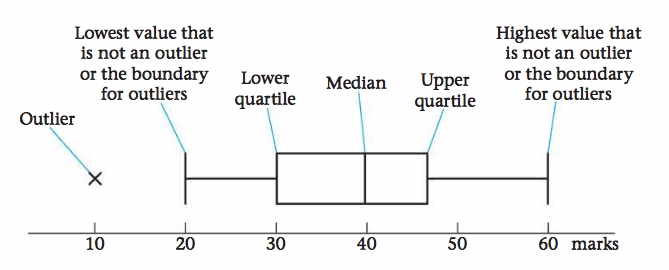
\includegraphics[scale=0.5]{img_S/4_intro}
\end{center}

\subsection{Histogram}

\begin{defi}[Frequency density]
	\[
		\text{frequency density}=\frac{\text{frequency}}{\text{class width}}
	\]
\end{defi}
\begin{eg}
	7
\end{eg}

\subsection{Skewness (Shape)}
A distribution can be symmetrical , have positive skew or have negative skew\\


symmetrical $Q_2-Q_1=Q_3-Q_2$ or mode$=$median$=$mean
\begin{center}
	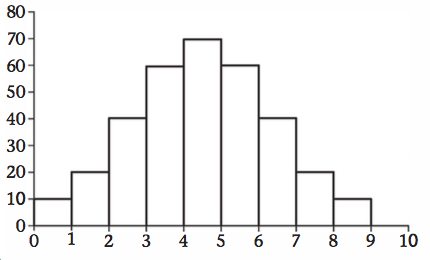
\includegraphics[scale=0.5]{img_S/3_5_intro1}
\end{center}
positive :$Q_2-Q_1<Q_3-Q_2$ or mode$<$median$<$mean
\begin{center}
	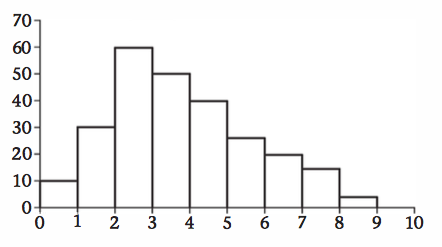
\includegraphics[scale=0.5]{img_S/3_5_intro2}
\end{center}
negative :$Q_2-Q_1>Q_3-Q_2$ or mode$>$median$>$mean
\begin{center}
	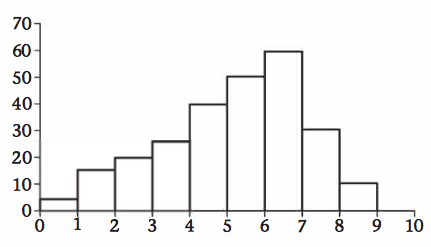
\includegraphics[scale=0.5]{img_S/3_5_intro3}
\end{center}

Or you can calculate:
\[
	\frac{3(\text{mean}-\text{median})}{\text{SD}}
\]


\subsection{What!?}
\begin{eg}
	example 10-12
\end{eg}
\section{Probability}
\subsection{Classical Probability}
\subsection{Venn diagram and their rules}
\begin{defi}[Complementary Probability]
\end{defi}
\subsection{Conditional Probabilites}
\subsubsection{Vann diagram}
\subsubsection{Tree diagram}
\subsection{Special Events of Probabilites}

\begin{defi}[Mutually exclusive]
	When events have no outcomes in common, they are mutually exclusive.
	\begin{center}
		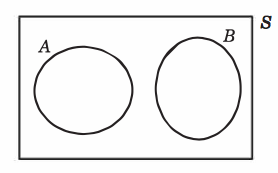
\includegraphics[scale=0.5]{img_S/4_6_intro}
	\end{center}

\end{defi}
There is no intersection of A and B, so $P(A\cap B)=0$\\

We can use $P(A\cup B)=P(A)+P(B)-P(A\cap B)$

result is
\[
	P(A\cup B)=P(A)+P(B)
\]

\begin{defi}[Independent events]
	When one event has no effect on another, they are independent so $P(A|B)=P(A)$
\end{defi}

by $\frac{P(A\cap B)}{P(B)}=P(A)$ we have:

\[
	P(A\cap B)=P(B)\times P(A)
\]



\section{Correlation}
\subsection{Correlation}
\begin{center}
	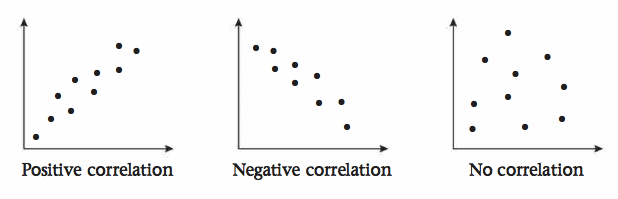
\includegraphics[scale=0.5]{img_S/5_1_intro}
\end{center}
\subsection{Bivariate data}
Recall this formula :
\[
	\text{Variance}=\frac{\sum (x-\bar{x})^2}{n}
\]
In correlation we write:
\[
	S_{xx}=\sum (x-\bar{x})^2
\]

\[
	S_{yy}=\sum (y-\bar{y})^2
\]

so
\[
	\text{Variance}=\frac{S_{xx}}{n}
\]

\begin{defi}[Co-Variance]
	\[
		S_{xy}=\frac{\sum(x-\bar{x})(x-\bar{y})}{n}
	\]
\end{defi}

\subsection{Product moment Correlation coefficient $r$}
\[
	r=\frac{S_{xy}}{\sqrt{S_{xx}S_{yy}}}
\]

The value of $r$ varies between -1 and 1\\

If $r=1$ , positive linear correlation\\

If $r=-1$, nagative linear correlation\\

If $r=0$, no linear correlation\\

limitation:

\subsection{Coding}
does not effect $r$
\section{Regression}
\subsection{Linear}
let $y=a+bx$ be a regression line \\
where
\[
	b=\frac{S_{xy}}{S_{xx}} \mbox{~and~} a=\bar{y}-b\bar{x}
\]
\subsection{Coding}
\subsection{Interpolation and Extrapolation}

\section{Discrete random variables}
\subsection{Probability distribution}

\begin{defi}[Mean / Expected value]
	\[
		E(X)=\sum xp(x)
	\]
\end{defi}
when we find $E(X^n)$:
\[
	E(X^n)=\sum x^np(x)
\]
\begin{defi}[Variable]
	\[
		Var(X)=E(X^2)-(E(X))^2
	\]
\end{defi}

The constant $a$ and $b$ affect on $E(X)$ and $Var(X)$
\[
	E(aX+b)=aE(x)+b
\]

\[
	Var(aX+b)=a^2Var(X)
\]
\begin{defi}[Uniform distribution]
	The distribution is uniform when all the probabilities is the same of all values.
\end{defi}


\section{The normal distribution}
$Z\sim  N(\mu,\sigma^2)$ represent the normal distribution.\\

\begin{center}
	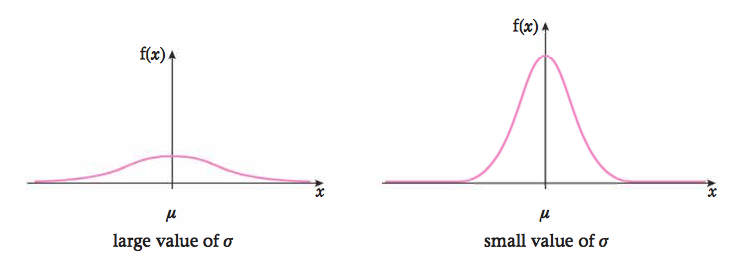
\includegraphics[scale=0.5]{img_S/8_intro}
\end{center}

The random variable $X$ can be written as $X\sim  N(\mu,\sigma^2)$\\

you can transformed $X$ to $Z$ by this formula
\[
	z=\frac{X-\mu}{\sigma}
\]
\begin{eg}
	Example 8-9
\end{eg}

\section{Binomial distribution}
\subsection{Basic Concept}
$X\sim B(n,p)$ represent the Binomial distribution, then
\[
	P(X=x)=\begin{pmatrix}n\\x\end{pmatrix}p^x(1-p)^{n-x}
\]

\subsection{Mean and Variance}
If $X\sim B(n,p)$ then
\begin{align*}
	E(X)   & =\mu=np           \\
	Var(X) & =\sigma^2=np(1-p)
\end{align*}

\begin{eg}
	example 9-14
\end{eg}
\section{Poisson distribution}
\subsection{Basic Concepts}
Recall the exponential function
\[
	e^x=1+\frac{x^1}{1!}+\frac{x^2}{2!}+\frac{x^3}{3!}+\cdots++\frac{x^r}{r!}+\cdots
\]
If you let $x=\lambda$ and remember that $\lambda^0=1$ this gives
\[
	e^{\lambda}=\lambda^0+\frac{\lambda^1}{1!}+\frac{\lambda^2}{2!}+\frac{\lambda^3}{3!}+\cdots++\frac{\lambda^r}{r!}+\cdots
\]
Dividing by $e^{\lambda}$ gives
\[
	\frac{e^{\lambda}}{e^{\lambda}}=\lambda^0+\frac{\lambda^1e^{-\lambda}}{1!}+\frac{\lambda^2e^{-\lambda}}{2!}+\frac{\lambda^3e^{-\lambda}}{3!}+\cdots+\frac{\lambda^re^{-\lambda}}{r!}+\cdots
\]
And the probability function is
\[
	P(X=x)=\frac{\lambda^xe^{-\lambda}}{x!}
\]
We say that $X$ has a Poisson distribution with parameter $\lambda$ abd write
\[
	X\sim Po(\lambda)
\]
\subsection{Mean and Variance}
\[
	Var(X)=E(X)=\mu=\sigma^2=\lambda
\]
\begin{lemma}
	If mean and standard deviation square is same, we usually use Poisson distribution.
\end{lemma}
\begin{eg}
	example 5-6
\end{eg}

\subsection{Approximate a Binomial with Poisson}
If $X\sim B(n,p)$ and\\
\begin{itemize}
	\item $n$ is large
	\item $p$ is small
\end{itemize}
then X can be approximated by
\[
	Po(np)
\]
\begin{eg}
	example 7-8 9-10
\end{eg}
\section{Continuous random variables}
\subsection{Continous random variable}
The Continuous random variables with p.d.f $f(x)$ satisfied the following properties:
\begin{enumerate}
	\item $f(x)\geq 0$ since we cannot have negative probabilities
	\item $P(a<X<b)= \text{shaded area} = \int_a^b f(x) \, \d x$
	      \begin{center}
		      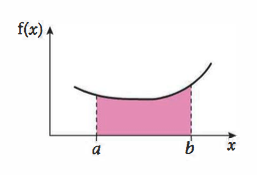
\includegraphics[scale=0.5]{img_S/11_1_intro1}
	      \end{center}
	\item  $\int_{-\infty}^{\infty}f(x)\, \d x=1$ since the area under the curve $=1$.
	      \begin{center}
		      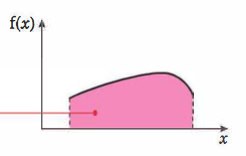
\includegraphics[scale=0.5]{img_S/11_1_intro2}
	      \end{center}
\end{enumerate}

\begin{eg}
	The random variable $X$ has probability density function
	\[
		f(x)=
		\begin{cases}
			kx(4-x) & 2\leq x \leq 4    \\
			0       & \text{otherwise.}
		\end{cases}
	\]
	Find the value of $k$ and sketch the p.d.f
	\begin{proof}
		\begin{align*}
			\int_2^4 k(4x-x^2)\, \d x & = 1             \\
			k[2x^2-\frac{x^3}{3}]_2^4 & =1              \\
			k                         & =(\frac{3}{16})
		\end{align*}
		\begin{center}
			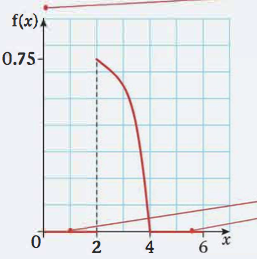
\includegraphics[scale=0.5]{img_S/11_2}
		\end{center}
	\end{proof}
\end{eg}

\begin{eg}
	The random variable $X$ has probability density function
	\[
		f(x)=
		\begin{cases}
			k      & 1<x<2             \\
			k(x-1) & 2\leq x \leq 4    \\
			0      & \text{otherwise.}
		\end{cases}
	\]
	Find the value of $k$ and sketch the p.d.f
	\begin{proof}
		\begin{align*}
			\int_1^2 k\, \d x+\int_2^4 k(x-1)\, \d x & =1           \\
			k                                        & =\frac{1}{5}
		\end{align*}
		\begin{center}
			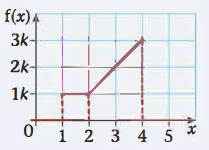
\includegraphics[scale=0.5]{img_S/11_3}
		\end{center}
	\end{proof}

\end{eg}
\subsection{Cumulative distribution function}
\[
	F(x)=P(X\leq x)=\int_{-\infty}^x f(t) \, \d t
\]
where $F(x)=P(X\leq x)=1$
\begin{center}
	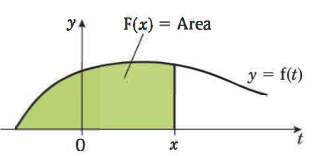
\includegraphics[scale=0.5]{img_S/11_2_intro}
\end{center}
If $X$ us a Continous random variable with c.d.f. $F(x)$ and p.d.f $f(x)$
\[
	f(x)=\frac{\d }{\d t} F(x) \mbox{~and~} F(x)=\int_{-\infty}^x f(t) \, \d t
\]

\begin{eg}
	example 5-6
\end{eg}
\subsection{Mean and Variance}
If $X$ is a Continuous random variable with p.d.f $f(x)$
\[
	\mu=E(X)=\int_{-\infty}^{\infty}x f(x) \, \d x
\]
\[
	\sigma^2=E(X^2)-\mu^2=\int_{-\infty}^{\infty}x^2 f(x) \, \d x-\mu^2
\]
\begin{remark}
	The range is the range of that function instead of negative infinity to infinity.
\end{remark}
\subsection{Mode, median and quartiles}
The median $m$ or $Q_2$ satisfies $F(m)=F(Q_2)=0.5$\\
The lower quartile $Q_1$ satisfies $F(Q_1)=0.25$ \\
The lower quartile $Q_1$ satisfies $F(Q_3)=0.75$ \\

The mode is the $x$ value at the highest point of the p.d.f $f(x)$

\section{Continuous uniform distribution}
\subsection{Continuous uniform distribution}
\begin{center}
	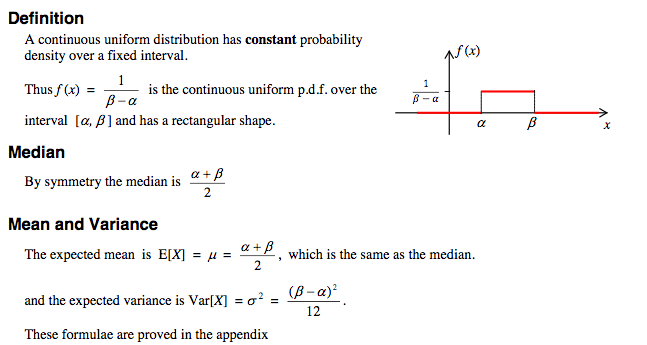
\includegraphics[scale=0.5]{img_S/12_intro}
\end{center}
\subsection{Mean and Variance}

\begin{eg}
	example 4-7

\end{eg}

\subsection{Choosing the right model}

\begin{eg}
	example 8-10
\end{eg}

\section{Normal approximation}
\subsection{Approximating binomial by normal}
If $X\sim B(n,p)$ and
\begin{itemize}
	\item $n$ is large
	\item $p$ is close to $0.5$
\end{itemize}
Then $X$ can be approximated by
\[
	Y\sim N(np,np(1-p))
\]

\begin{eg}
	$X\sim B(120,0.25)$ approximated to $Y\sim N(30,(\sqrt{22.5})^2)$
\end{eg}

\begin{eg}
	example 4
\end{eg}

\subsection{Approximating Poisson by normal}
If $\lambda$ is large
\[
	X\sim Po(\lambda) \text{to} Y\sim N(\lambda,(\sqrt{\lambda})^2)
\]

\begin{eg}
	$X\sim Po(25)$ transformed to $Y\sim N(25,5^2)$
\end{eg}

\begin{eg}
	example 6
\end{eg}

\subsection{Choosing the appropriate approximation}
\begin{center}
	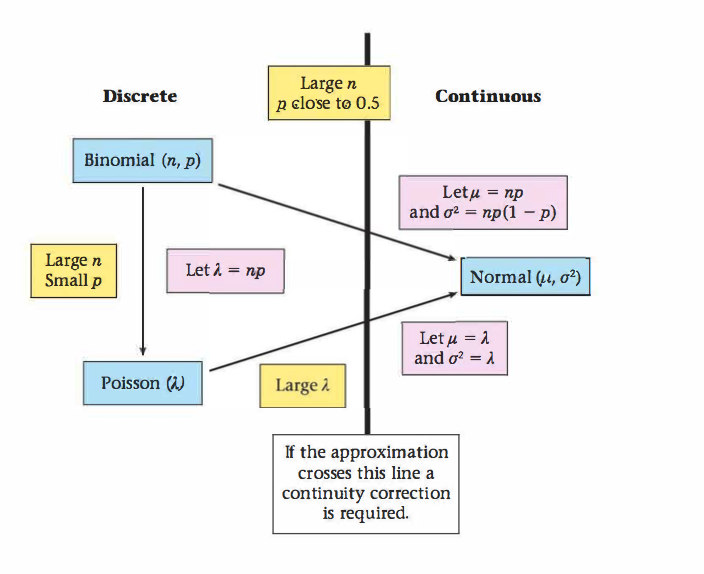
\includegraphics[scale=0.5]{img_S/13_3_intro}
\end{center}
\begin{eg}
	example 7
\end{eg}

\section{Population and samples}

\subsection{The Concept of population and samples}
List of the possible samples and find their probabilities and distribution.
\begin{eg}
	example 5 6
\end{eg}

\section{Hypothesis testing}
\subsection{Concept of hypothesis testing}
\begin{defi}[Null hypothesis $H_0$]
	The hypothesis which is assumed to be correct unless shown otherwise.
\end{defi}
\begin{defi}[Alternarive hypothesis $H_1$]
	This is the conclusion that should be made if $H_0$ is rejected
\end{defi}

\begin{defi}[Critical region]
	The range of values which would lead you to reject the null hypothesis, $H_0$
\end{defi}

\begin{defi}[Significance level]
	The actual significance level is the probability of rejecting $H_0$ when it is in fact true.
\end{defi}
From your observed result (test statistic) you decide whether to reject or not to reject the null
hypothesis $H_0$
\begin{center}
	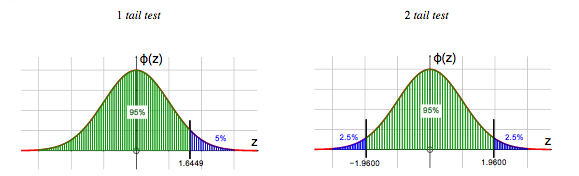
\includegraphics[scale=0.5]{img_S/15_intro}
\end{center}

The test statistic is significantat 5\%, or that we reject $H_0$. Thus $H_0$could actually be true but we still reject it.
Thus, the significance level, 5\%, is  \\
the probability that we reject $H_0$ when it is in fact true, or the probability of incorrectly rejecting $H_0$.\\
When we reject the null hypothesis, $H_0$, we use the alternative hypothesis to write the conclusion.\\


The Poisson and Binomial distributions are
discrete, and we look at probability histograms.

\begin{center}
	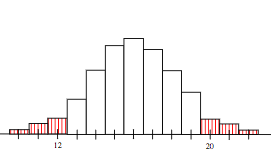
\includegraphics[scale=0.5]{img_S/15_intro2}
\end{center}

In the diagram, the critical region (shown by the
shaded areas) is $X\leq 12$ or $X\geq 20$.\\

We include the whole bar around $X=12$ and around $X=20$\\

So $P(X\leq 12)$ is the area to the left of 12.5,\\
and $P(X\geq 20)$ is the area to the right of 19.5,\\

If $P(X\leq 12)=0.0234$ and $P(X\geq 20)=0.0217$, then \\
the actual signifaicance level is $0.0234+0.0217=0.0451=4.51\%$ \\
Thus the probability of incorrectly rejecting $H_0$ is 0.0451.
\subsection{One- and two-tailed tests}
The One-tail test is
\begin{align*}
	H_0: & a=b                 \\
	H_1: & a>b \mbox{~or~} a<b
\end{align*}
The Two-tail test is
\begin{align*}
	H_0: & a=b     \\
	H_1: & a\neq b
\end{align*}
\begin{eg}
	3
\end{eg}

\begin{eg}
	4-13
\end{eg}

\section{Combination of random variables}
If $X_1$ and $X_2$ are independent normal random variables
\[
	X_1 \sim \N(\mu_1,\sigma_1^2) \mbox{~and~} X_2 \sim \N(\mu_2,\sigma_2^2)
\]
then $X_1+X_2$ and $X_1-X_2$ are also normal random variables
\[
	X_1+X_2\sim \N(\mu_1+\mu_2,\sigma_1^2+\sigma_2^2) \mbox{~and~} X_1-X_2\sim \N(\mu_1-\mu_2,\sigma_1^2+\sigma_2^2)
\]


\section{Estimation , confidence intervals and tests}
\subsection{Estimation}
\begin{defi}[Biased and unbiased estimator]
	If $X$  (usually found from a sample) is used to estimate the value of a population parameter,
	$t$, then $X$ is an unbiased estimator of $t$ if $E[X] =$ the true value of the parameter $t$. \\

	If an estimator, $X$, is biased, then the bias is the difference between $E[X]$ and the true value of the parameter $t$.
\end{defi}

\begin{defi}[Unbiased estimators of $\mu$ and $\sigma^2$]

\end{defi}


\subsection{Confidence intervals and significance tests}
\begin{defi}[Sampling distribution of the mean]
	\[
		\N(\mu,\frac{\sigma^2}{n})
	\]
\end{defi}

\begin{thm}[Central limit theorem]
	If $\{X_1,X_2,\cdots,X_n\}$ is a random sample of size $n$ drawn any population with mean $\mu$ and variance $\sigma^2$ then the population of sample means.
	\begin{enumerate}
	\item has expected mean $\mu$
	\item has expected variance $\frac{\sigma^2}{n}$
	\item forms a normal distribution if $n$ is 'large enough' i.e. $\bar{X}\sim \N(\mu,\frac{\sigma^2}{n})$
	\end{enumerate}
	The standard error of the sample mean is $\frac{\sigma}{\sqrt{n}}$
\end{thm}

\begin{eg}
\end{eg}
\begin{center}
	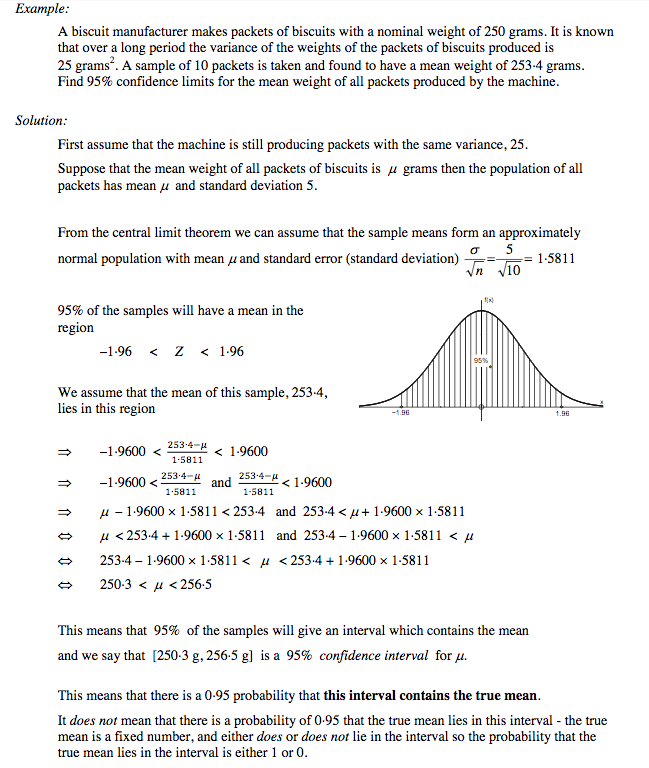
\includegraphics[scale=0.5]{img_S/18_eg1_1}
\end{center}
\begin{center}
	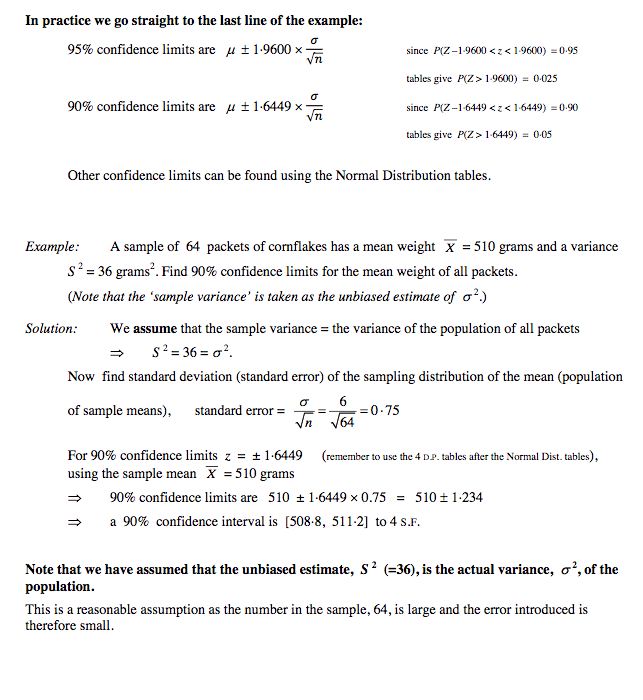
\includegraphics[scale=0.5]{img_S/18_eg1_2}
\end{center}


\begin{eg}
\end{eg}
\begin{center}
	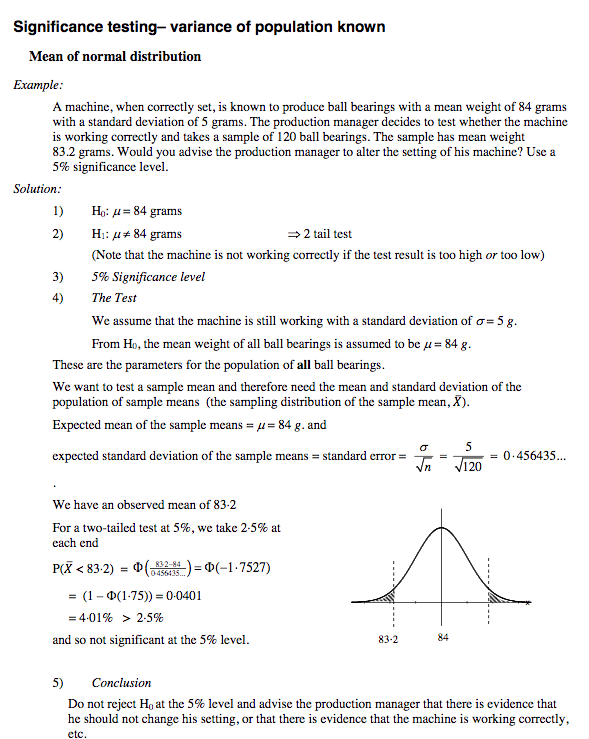
\includegraphics[scale=0.5]{img_S/18_eg2}
\end{center}

Fortunately the formula for testing the difference between sample means 
\[
	Z=\frac{\bar{X}-\bar{Y}-(\mu_x-\mu_y)}{\sqrt{\frac{\sigma_x^2}{n_x}+{\frac{\sigma_y^2}{n_y}}}}
\]
is in your formula booklet

\subsection{Combination of sampling distribution}
Same

\section{Goodness of fit and contingency tables}
\subsection{Basic Concept}
\begin{defi}[$\chi$ test]
	\[
		\chi^2=\sum\frac{(O_i-E_i)^2}{E_i}
	\]
where $O_i$ and $E_i$ are the observed and expected frequencies
\end{defi}

\subsection{Examples for all distributions}
\begin{center}
	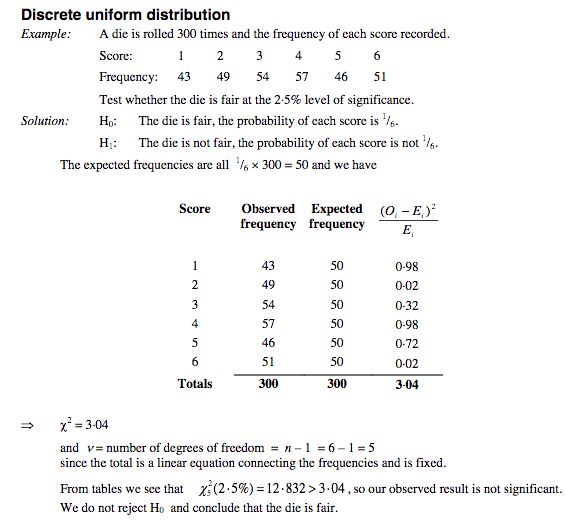
\includegraphics[scale=0.5]{img_S/19_eg1}
\end{center}
\begin{center}
	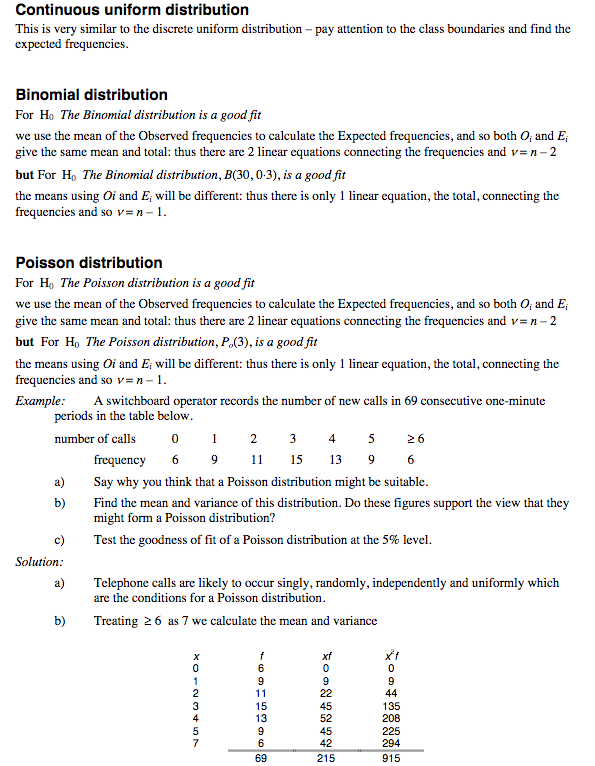
\includegraphics[scale=0.5]{img_S/19_eg2}
\end{center}
\begin{center}
	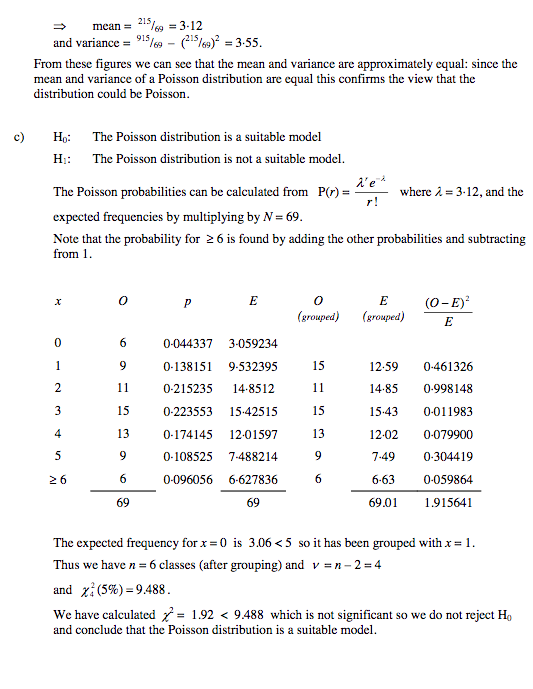
\includegraphics[scale=0.5]{img_S/19_eg3}
\end{center}
\begin{center}
	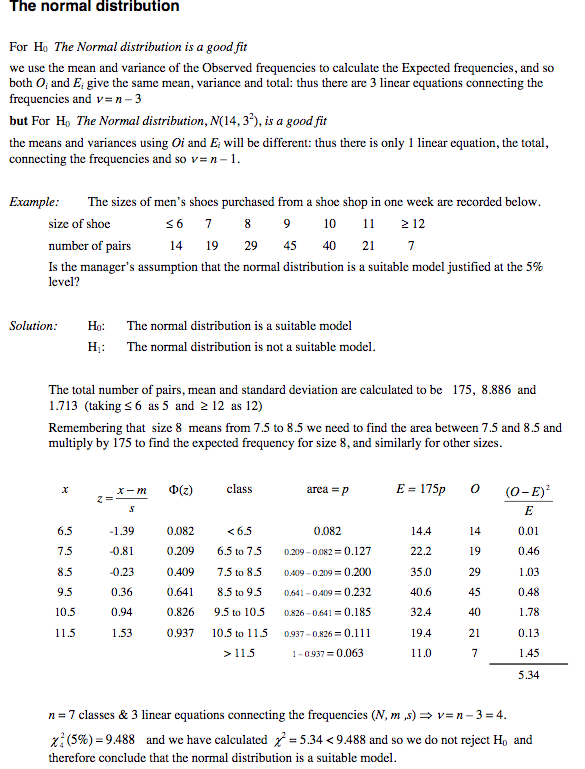
\includegraphics[scale=0.5]{img_S/19_eg4}
\end{center}
\begin{center}
	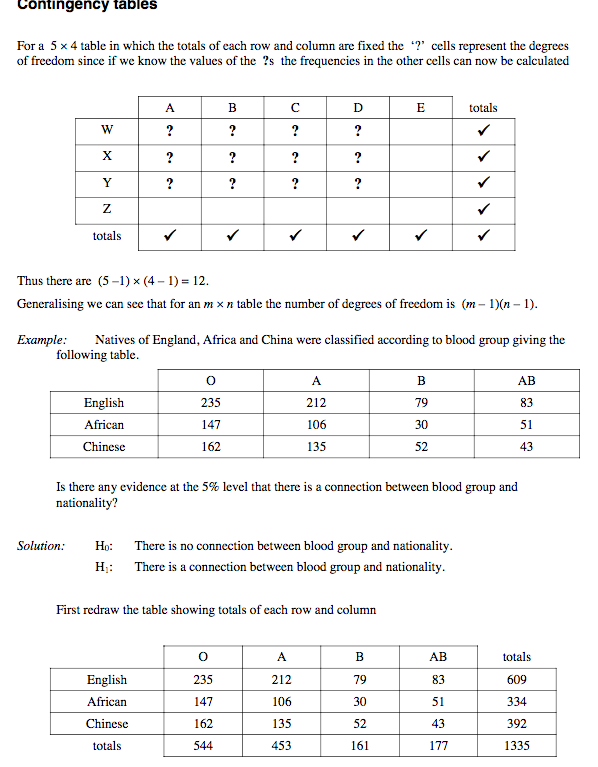
\includegraphics[scale=0.5]{img_S/19_eg5}
\end{center}
\begin{center}
	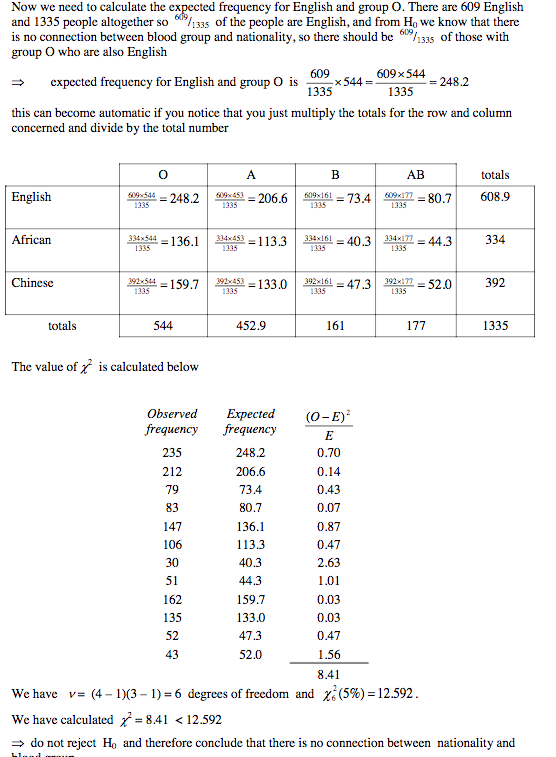
\includegraphics[scale=0.5]{img_S/19_eg6}
\end{center}



\section{Regression and correlation}
\begin{center}
	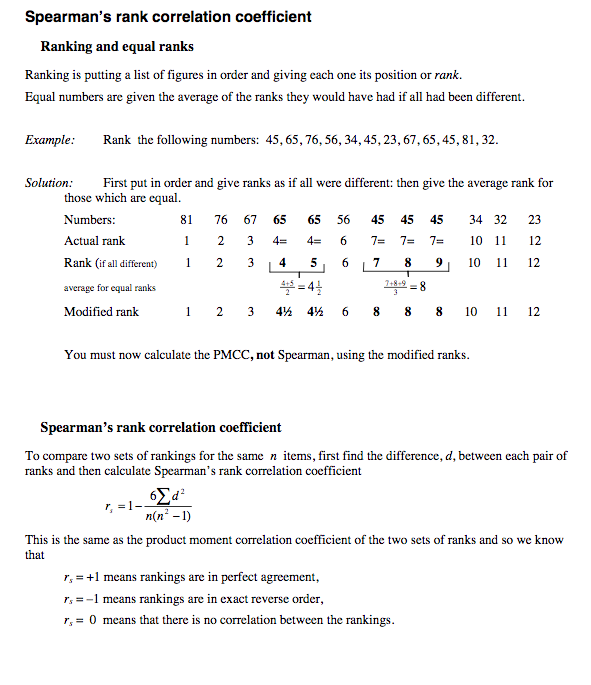
\includegraphics[scale=0.5]{img_S/20_eg1}
\end{center}
\begin{center}
	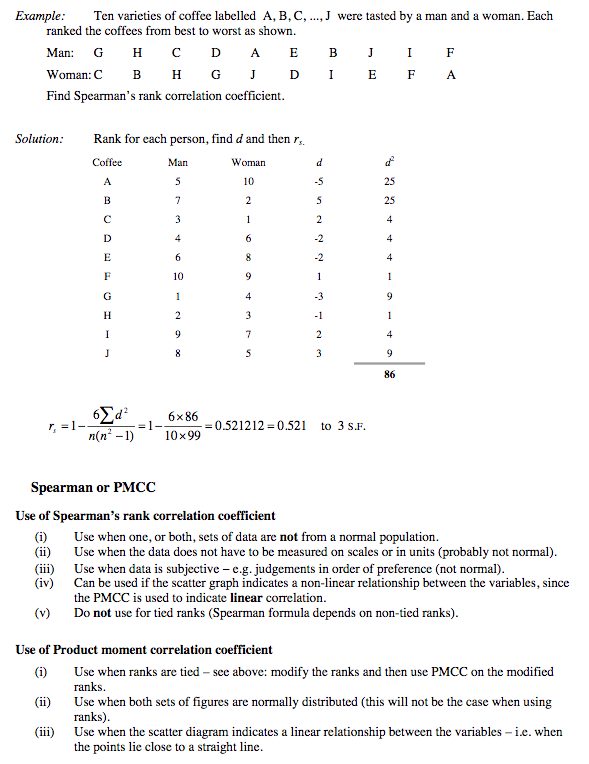
\includegraphics[scale=0.5]{img_S/20_eg2}
\end{center}
\begin{center}
	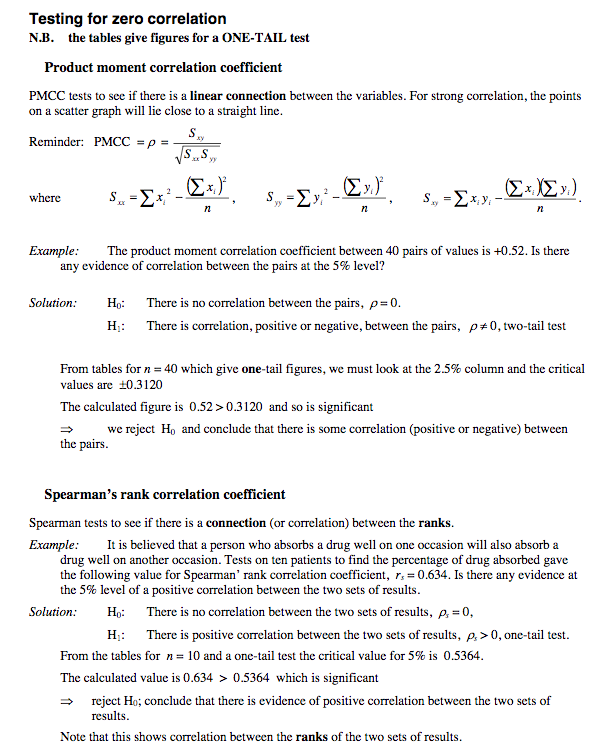
\includegraphics[scale=0.5]{img_S/20_eg3}
\end{center}
\begin{center}
	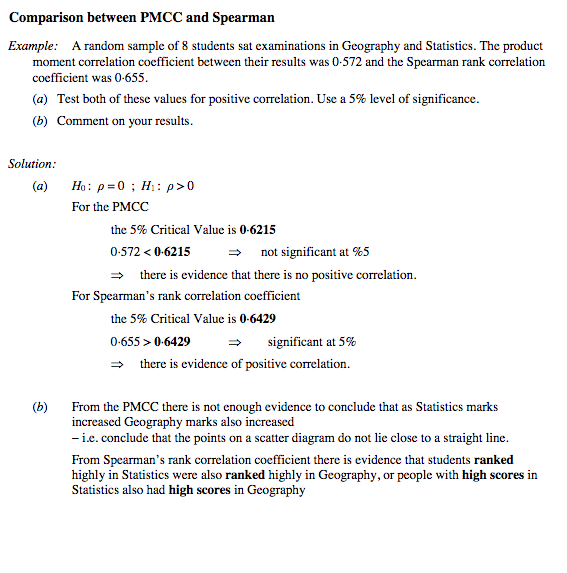
\includegraphics[scale=0.5]{img_S/20_eg4}
\end{center}


\section{Quality of tests and estimators}

\section{One-sample procedures}

\section{Two-sample procedures}

\printindex




\end{document}}